\documentclass{article}
\usepackage{graphicx}
\usepackage{amsmath}
\usepackage{amsfonts}
\usepackage{bookmark}
\usepackage{booktabs}
\usepackage{exercises}
\graphicspath{ {./images/5.7} }
\usepackage{indentfirst}
\usepackage{amsthm}
\usepackage{yhmath}
\usepackage{geometry}
\usepackage{placeins}
\usepackage{csquotes}
\usepackage{pgfplots}
\newcommand*{\oldneg}{\mathord{\sim}}
\newcommand\showdiv[1]{\overline{\smash{)}#1}}
\newcommand\Mydiv[1]{%
\smash{\raise.3ex\hbox{$\big)$}}\mkern-8mu
        \overline{\enspace\strut#1}}
\setlength{\tabcolsep}{5pt}
\theoremstyle{definition}
\newtheorem{definition}{Definition}

\setlength{\parindent}{.5in}
\setlength{\parskip}{12pt}
\renewcommand{\arraystretch}{2}
\geometry{margin=1in}
\newcommand{\?}{\stackrel{?}{=}}
\pgfplotsset{width=7cm,compat=1.18}\usepgfplotslibrary{statistics}

\title{5.7 Answers}
\begin{document}
\maketitle

\section*{1}
A function $f$ is an even function if $f(-x)=f(x)$ for all values of $x$ in the domain of $f$.

\section*{2}
Suppose we are given a domain $[a,b]$. We can determine whether the function $f$ over this domain is increasing or decreasing in the following way. We know that a function is increasing over the domain 
if, for all $x_1<x_2$ in the domain, $f(x_1)<f(x_2)$, and is decreasing if, for all $x_1<x_2$ in the domain, $f(x_1)>f(x_2)$. Thus, the way in which one can test if a function is increasing or decreasing is by 
considering any pair of points $x_1,x_2$ in the domain such that $x_1<x_2$. If it can be concluded that $f(x_1)<f(x_2)$, then the function is increasing, whereas, if it can be concluded that 
$f(x_2)<f(x_1)$, then the function is decreasing.

\section*{6}
We are comparing the rates of change over the provided intervals. The first interval, $[-4,-3]$, has a rate of change of \[ \dfrac{(3^{-3+4}-6)-(3^{-4+4}-6)}{-3+4}=2 \] The second 
interval, $[-3,-2]$, has a rate of change of \[ \dfrac{(3^{-3+4}-6)-(3^{-2+4}-6)}{-3+2}=6 \] The third interval, $[-2,-1]$, has a rate of change of
\[ \dfrac{(3^{-2+4}-6)-(3^{-1+4}-6)}{-2+1}=18 \] The fourth interval, $[-1,0]$, has a rate of change of
\[ \dfrac{(3^{-1+4}-6)-(3^{0+4}-6)}{-1+0}=54 \] The four provided intervals compare values of $x$ for which $x$ increases. From the computed rates of change in the given intervals, we can infer that the graph of the function 
increases as $x$ increases.

\section*{10}
In fact, the absolute value of the average rate of change decreases, but does not increase. This is because the average rate of change decreases in the negative direction, 
meaning the absolute value increases in the positive direction.

\section*{11}
We are given a function $f(x)$ and an interval $|x_1,x_2|$. We are given particular values of $x_2$ and $x_1$ such that $x_2>x_1$ and $f(x_2)>f(x_1)$. 
Recall that the definition of an increasing function is such that, for all $x_2>x_1$, $f(x_2)>f(x_1)$. 
Even though we know that $f(x_2)>f(x_1)$, it could be that there is some $x_3$ such that $x_2\ne x_3>x_1$ in the interval $|x_1,x_2|$ such that $f(x_3)<f(x_1)$. Thus 
we cannot conclude that $f(x)$ is increasing over the interval $|x_1,x_2|$.

\section*{14}
D

\section*{15}
Odd.

\section*{16}
Neither.

\section*{17}
Even.

\section*{21}
To determine if the function is even or odd, we need to compute the value of $k(-x)$:
\[ k(-x)=5(-x)^6+9(-x)^4+(-x)^2=5x^6+9x^4+x^2 \] meaning the function is even, as $k(x)=k(-x)$.

\section*{22}
To determine if the function is even or odd, we need to compute the value of $m(-x)$:
\[ m(-x)=\frac{12}{-x}=-\frac{12}{x} \] meaing the function is odd, as $k(-x)=-k(x)$.

\section*{23}
To determine if the function is even or odd, we need to compute the value of $m(-x)$:
\[ m(-x)=\frac{3}{-x}+5=-\frac{3}{x}+5 \] This means the function is neither even nor odd. For example, $m(-1)=-\frac{3}{1}+5=2$ and $m(1)=\frac{3}{1}+5=8$, that is, 
neither $k(x)=k(-x)$ or $k(-x)=-k(x)$.

\section*{24}
\[ g(-x)=11(-x)^6+7(-x)^2=11x^6+7x^2 \]
A

\section*{25}
(a): Suppose that two functions $f(x)$ and $g(x)$ are even. Thus $f(-x)=f(x)$ and $g(-x)=g(x)$. Consider their product $h(x)=f(x)\times g(x)$. 
We know that $h(-x)=f(-x)\times g(-x)=f(x)\times g(x)=h(x)$, meaning $h(x)$ is even. Thus the statement is always true.


(b): Suppose that two functions $f(x)$ and $g(x)$ are odd. Thus $f(-x)=-f(x)$ and $g(-x)=-g(x)$. Consider their product $h(x)=f(x)\times g(x)$. We know that 
$h(-x)=f(-x)\times g(-x)=-f(x)\times -g(x)=f(x)\times g(x)=h(x)$, meaning $h(x)$ is even, not odd. Thus the statement is never true. 

\section*{30}
This could be, for example, a situation in which a plane is making its descent. At first it might decline more rapidly, but as it gets closer to landing, it will approach a rate of change of zero.

\section*{31}
(a): The first pattern can be given by the function $f(x)=x^4$ where $x$ is the position of the number in the pattern and $f(x)$ is that number. The second pattern can be given by the 
function $g(x)=4^x$ where $x$ is the position of the number in the pattern and $g(x)$ is that number.


(b): \newline 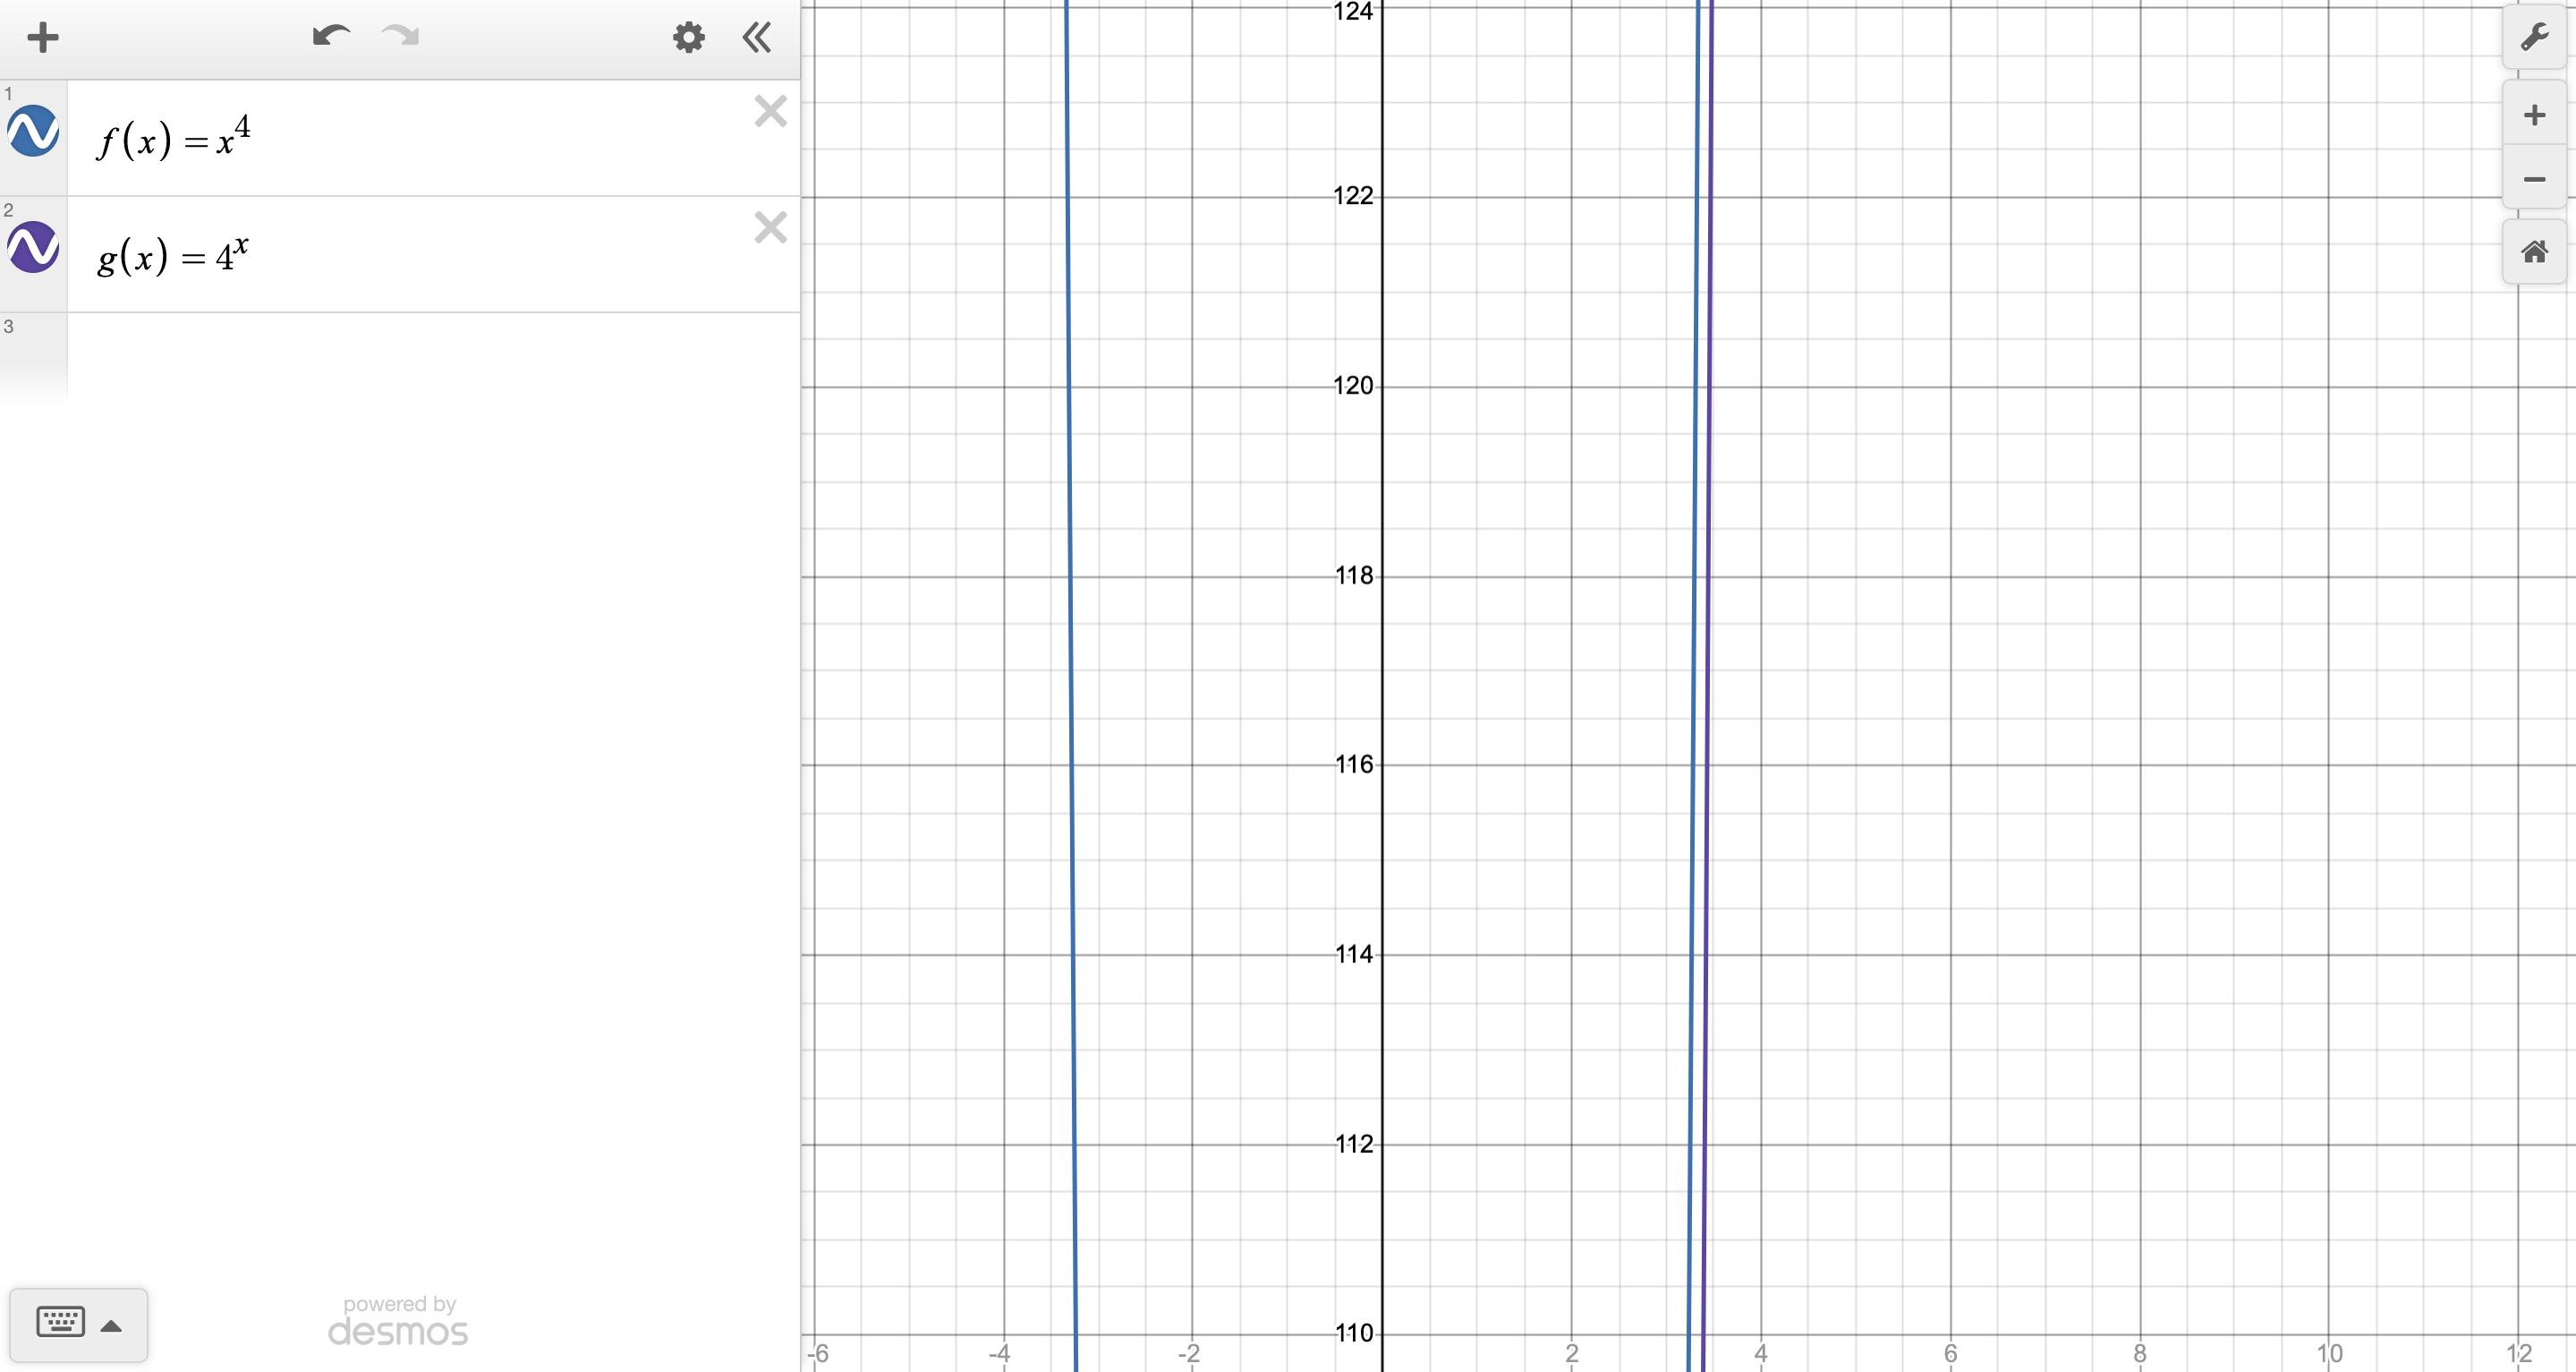
\includegraphics[width = 4in, height = 4in]{31a}\newline \newline 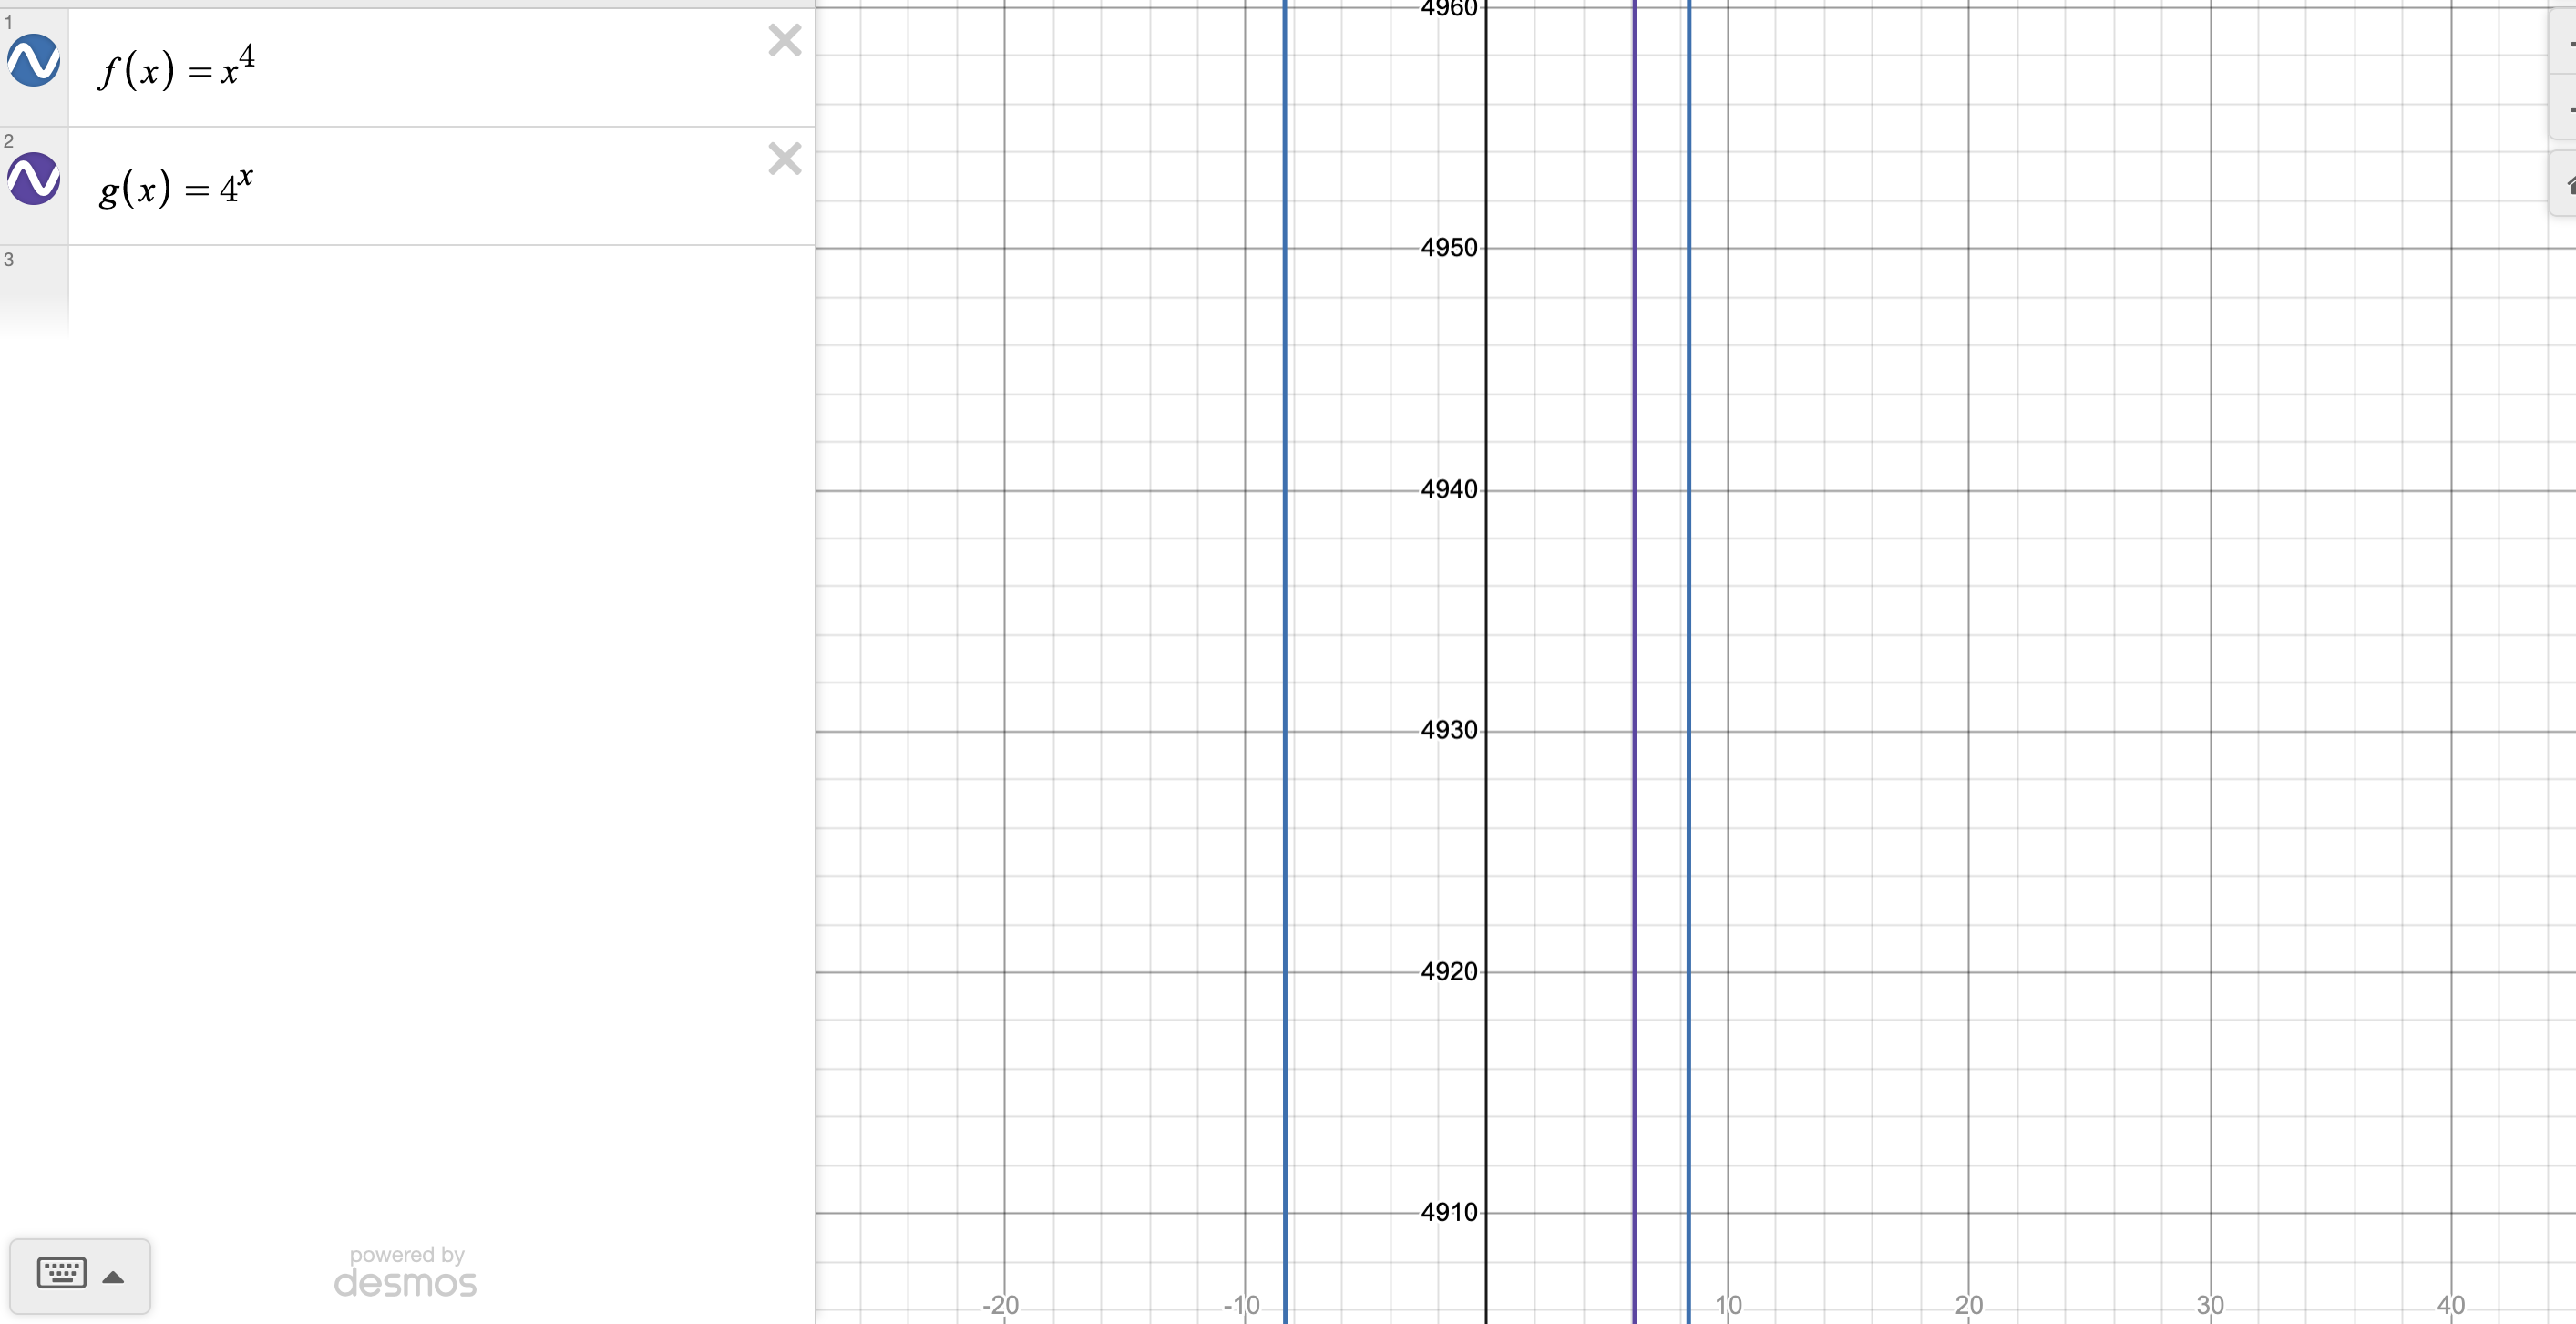
\includegraphics[width = 4in, height = 4in]{31b}\newline Just from looking at the graphs, there is no way to tell if one of the graphs 
eventually exceeds and increases more rapdily than the value of the other. For example, the graph of $x^4$ exceeds the graph of $4^x$ in the first picture, but the graph of $4^x$ exceeds the graph of $x^4$ in the second 
picture. However, we can give an algebraic justification that $4^x$ eventually exceeds $x^4$ in the following way. $4^x=x\log 4$ and 
$x^4=4\log x$. Because the rate of change of $\log x$ decreases as $x$ increases, and the rate of change of $x\log 4$ is linear, 
eventually, $x\log 4$ (that is, $4^x$) will exceed $4\log x$.


(c): A similar justification can be given to that as in part (b), showing that the expontential functions will eventually exceed polynomial functions. 

\end{document}
